\documentclass[12pt,a4paper]{article}
\usepackage[utf8]{inputenc}
\usepackage{graphicx}
\usepackage[none]{hyphenat}
\usepackage{hyperref}
\usepackage{xcolor}

\setlength{\fboxrule}{2pt}

\begin{document}
	\begin{titlepage}
		
		\begin{center}
			
\includegraphics[width=0.5\textwidth]{QUT.jpg}\\
			[0.03\textheight]  
			\Large\textbf{Bachelor of IT (Computer Science)}\\
			\Large\textbf{Assignment 2 - Client-Side React Application}\\
			\large\textbf{CAB230 - Web Computing}\\
			[0.02\textheight]
			\large\textsl{Dane Madsen}\\
			\large\textsl{n10983864@qut.edu.au}
		\end{center}
		
	\end{titlepage}
	\tableofcontents
	\newpage
	
	\section{Introduction}
		\subsection{Purpose and Description}
			The purpose of this react application is to collate and display information regarding movies, 
			and cast members to the user in a responsive and accessible manner. The application should 
			allow the user to search for movies by year or title and display the results in a list. 
			When a movie is selected, the application should display all the details of the movie, 
			including the year the movie was made, the plot of the movie and all the cast members 
			involved with the movie. The application should also allow the user to visit individual 
			pages of cast members where the user can view that cast members details, including their 
			birth year, death year and all the movies they have been involved with.\\
			\\
			It achieve this goal and to provide the user with the best experience I can, i have used a 
			number of advanced react features, including the use of react router, IntesectionObserver and 
			react-responsive-carousel. The use of these features has allowed me to create a 
			professional looking application that is both easy to use and responsive for the user.\\

			\begin{center}
				\fbox{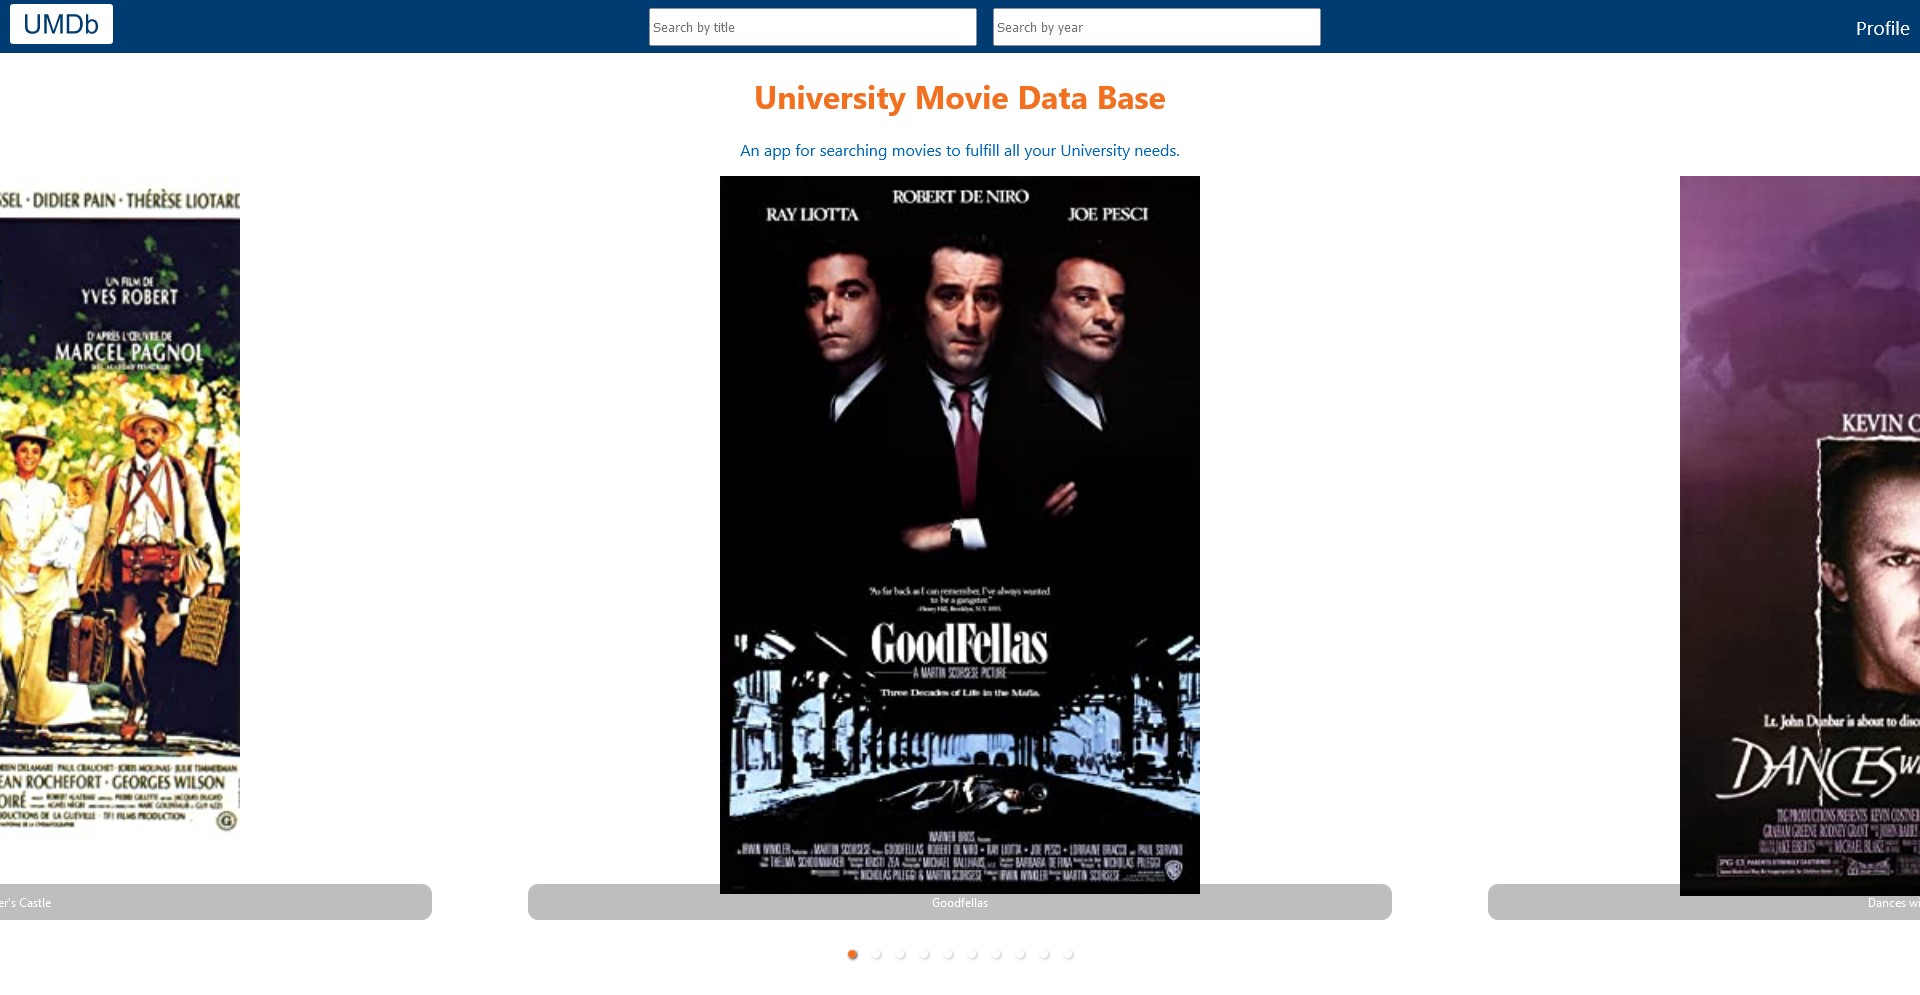
\includegraphics[width=\textwidth]{Figure1.jpg}}
				\fbox{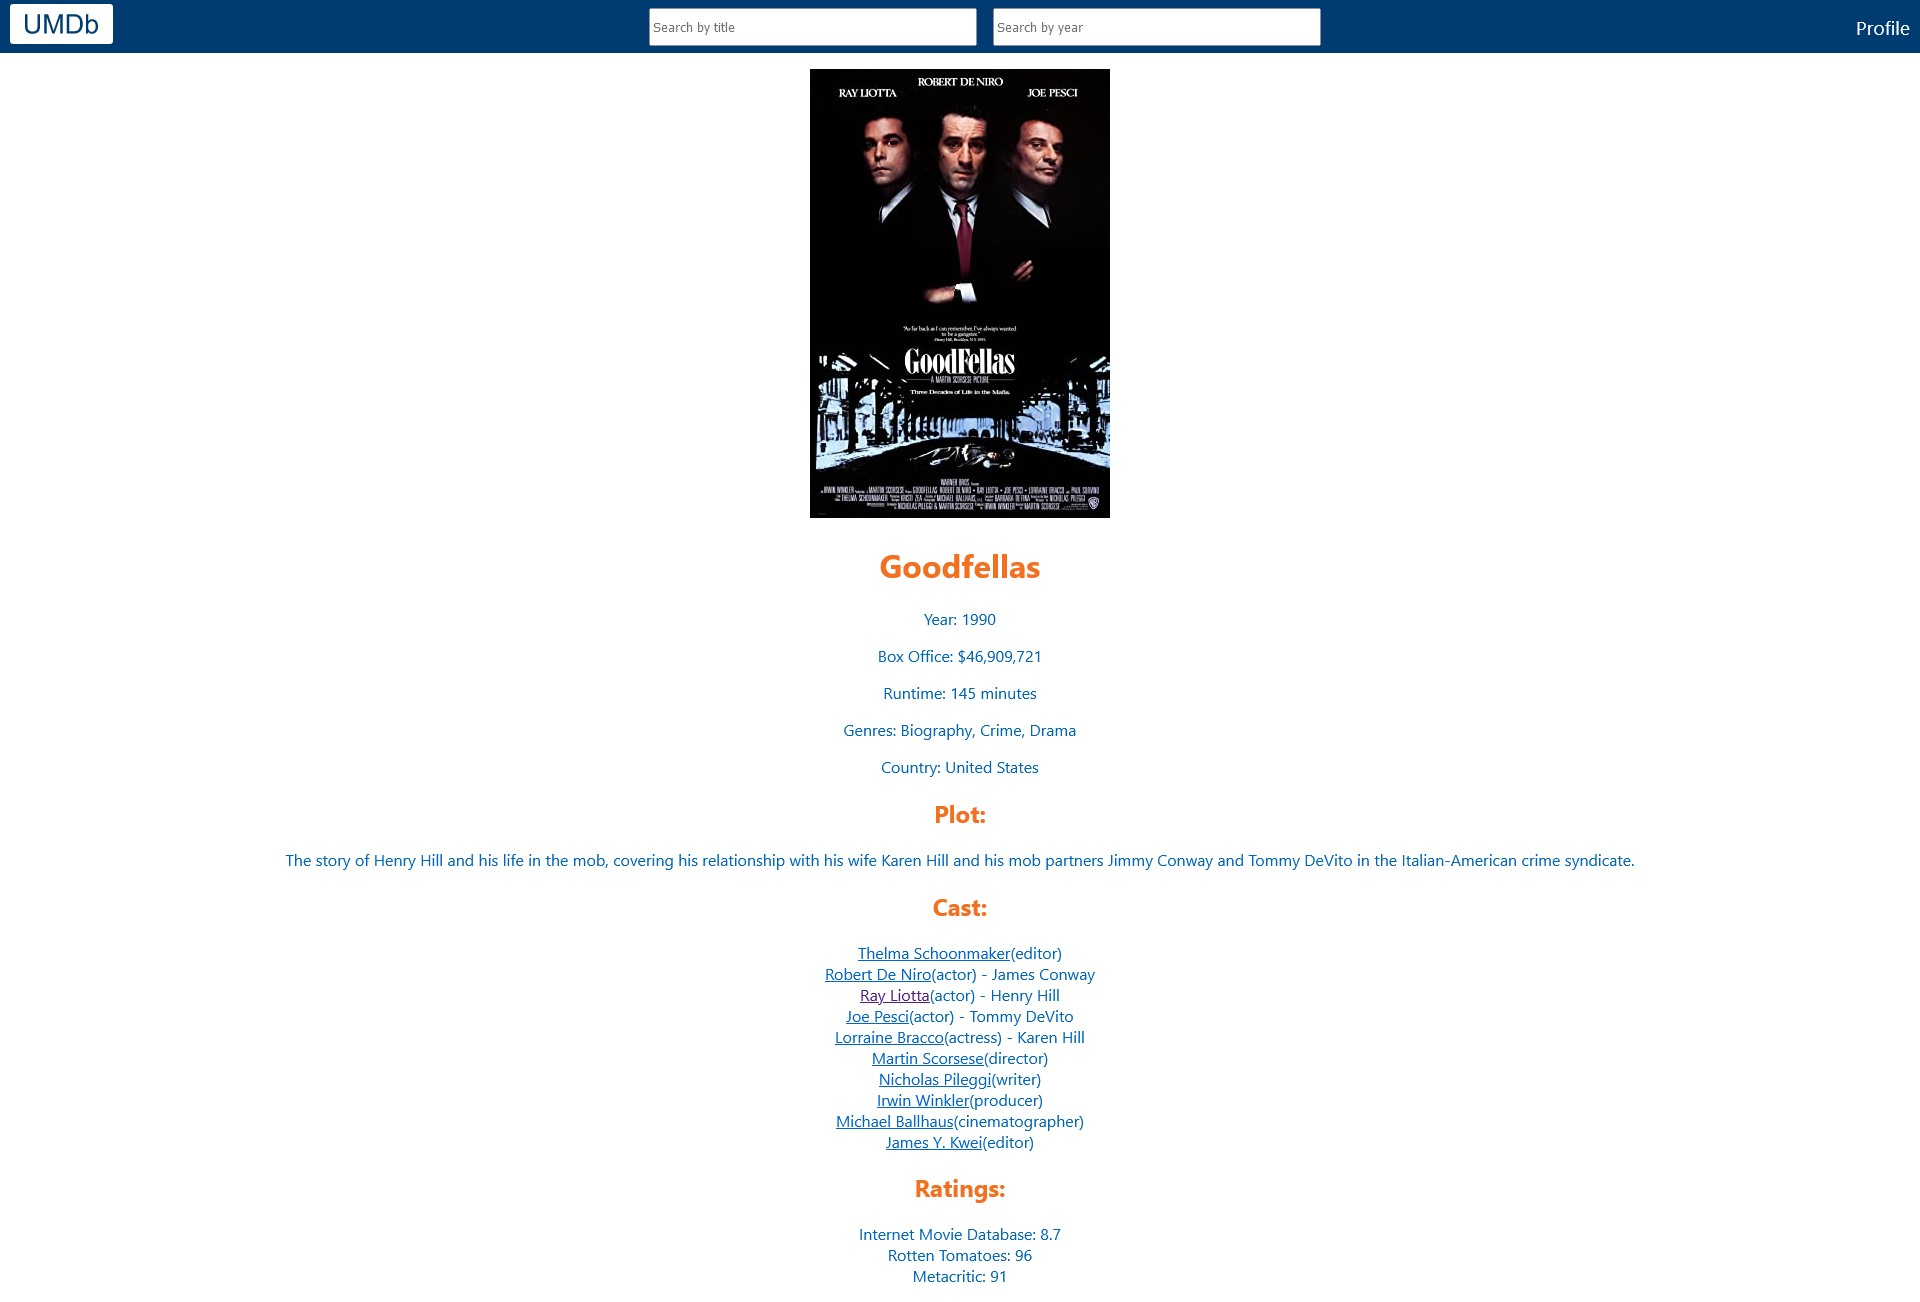
\includegraphics[width=\textwidth]{Figure2.jpg}}
			\end{center}
		
		\subsection{Completeness and Limitations}
			This implementation covers all the requirements of the assignment specification. 
			Navigation is handled using react router, controlled forms are used for all user input, and 
			every 10 minutes the refresh token is used to get a new access token. In addition to this, 
			the application uses ag-grid to display the search results in an infinitly scrolling grid 
			and react-responsive-carousel to display the highest scoring movies of all time on the 
			home (landing) page. On the person page the movies the person is involved in are displayed 
			in a grid with the IMDb Rating.\\

	\newpage

	\section{Use of End Points}
		\subsection{/movies/search}
			This endpoint is utilised by two search forms at the top of the application. The first 
			search form is for the user to search for movies by title, and the second is for the user 
			to search for movies by year. Both of these forms are controlled forms and can be accessed 
			from any page in the application. Doing it this way removes an extra layer of complexity for 
			the user and allows them to get into the function of the application right from the start of
			the application.\\

			\begin{center}
				\fbox{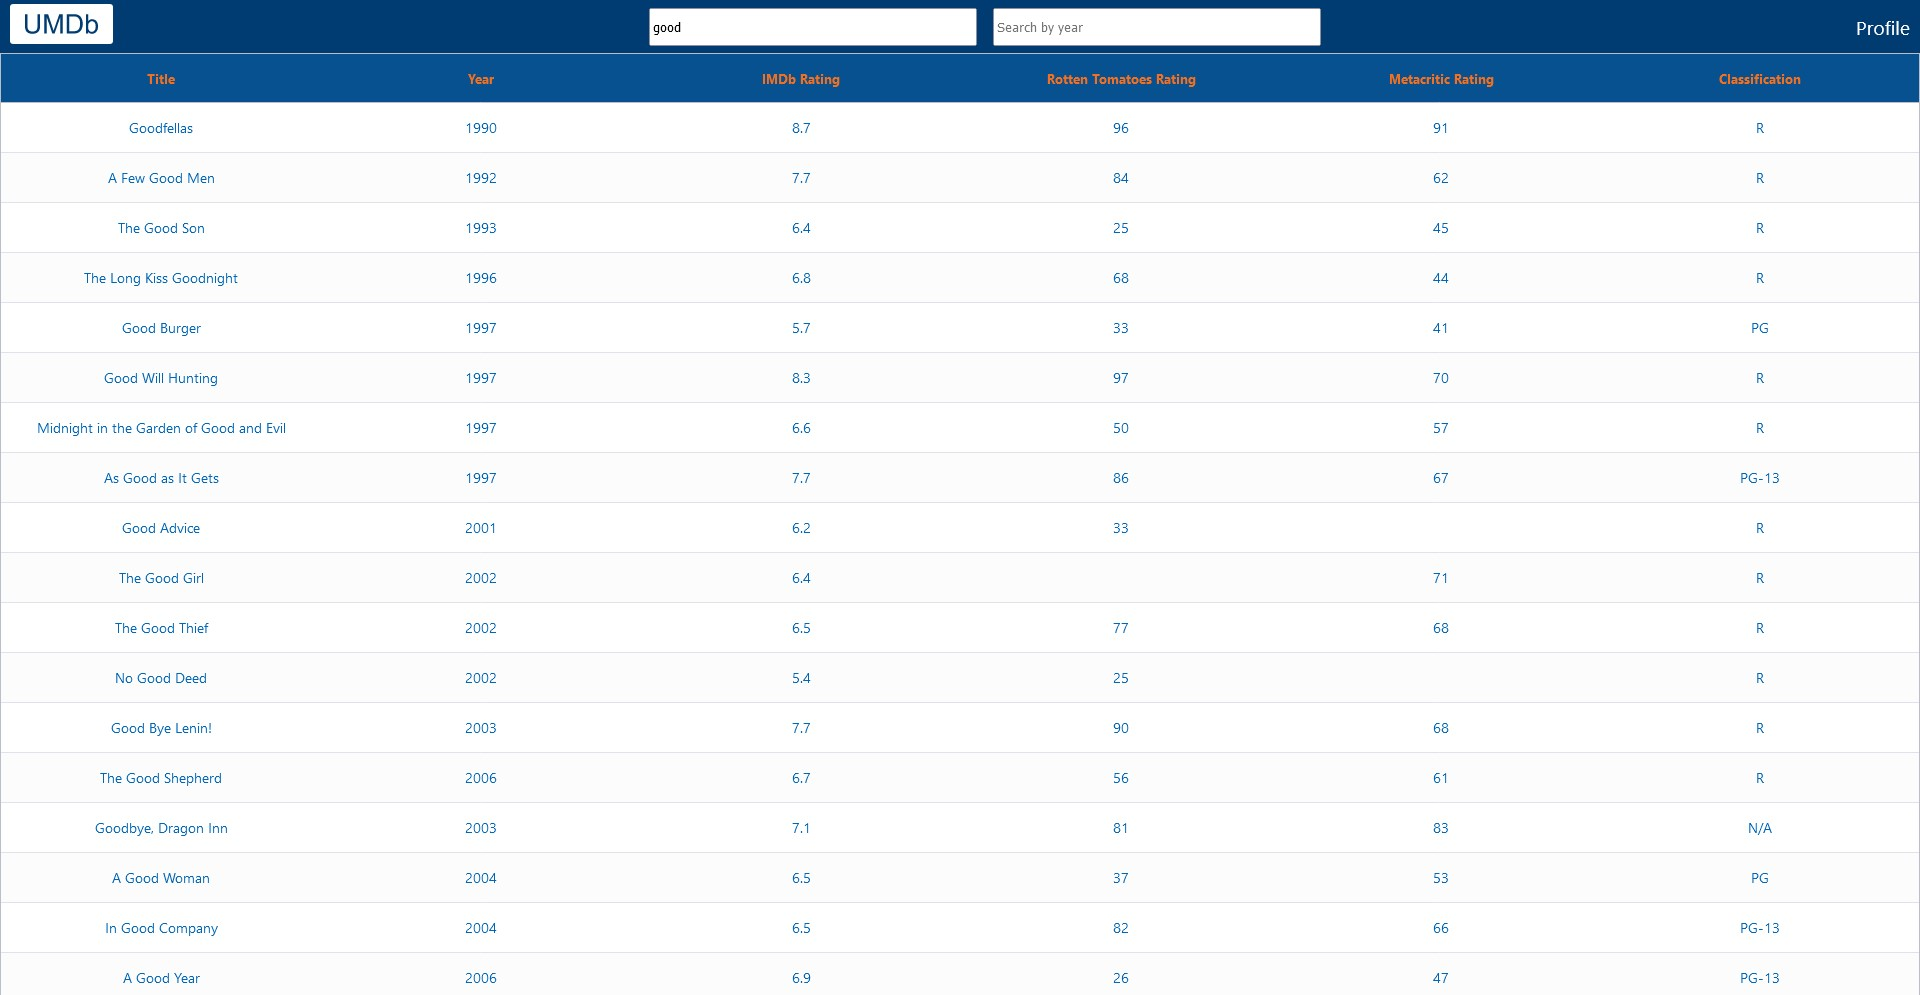
\includegraphics[width=\textwidth]{Figure3.jpg}}
			\end{center}

		\newpage

		\subsection{/movies/data/\{imdbID\}}
			This endpoint is utilised by the movie page to get the details of the movie the user has 
			selected. The movie page is accessed by clicking on any of the movies in the search results. 
			The movie page displays all the details of the movie, including the title, year, box office 
			earnings, runtime, genre, country of origin, plot, cast and ratings. each cast member is a 
			clickable link that will lead to that cast members respective page.\\

			\begin{center}
				\fbox{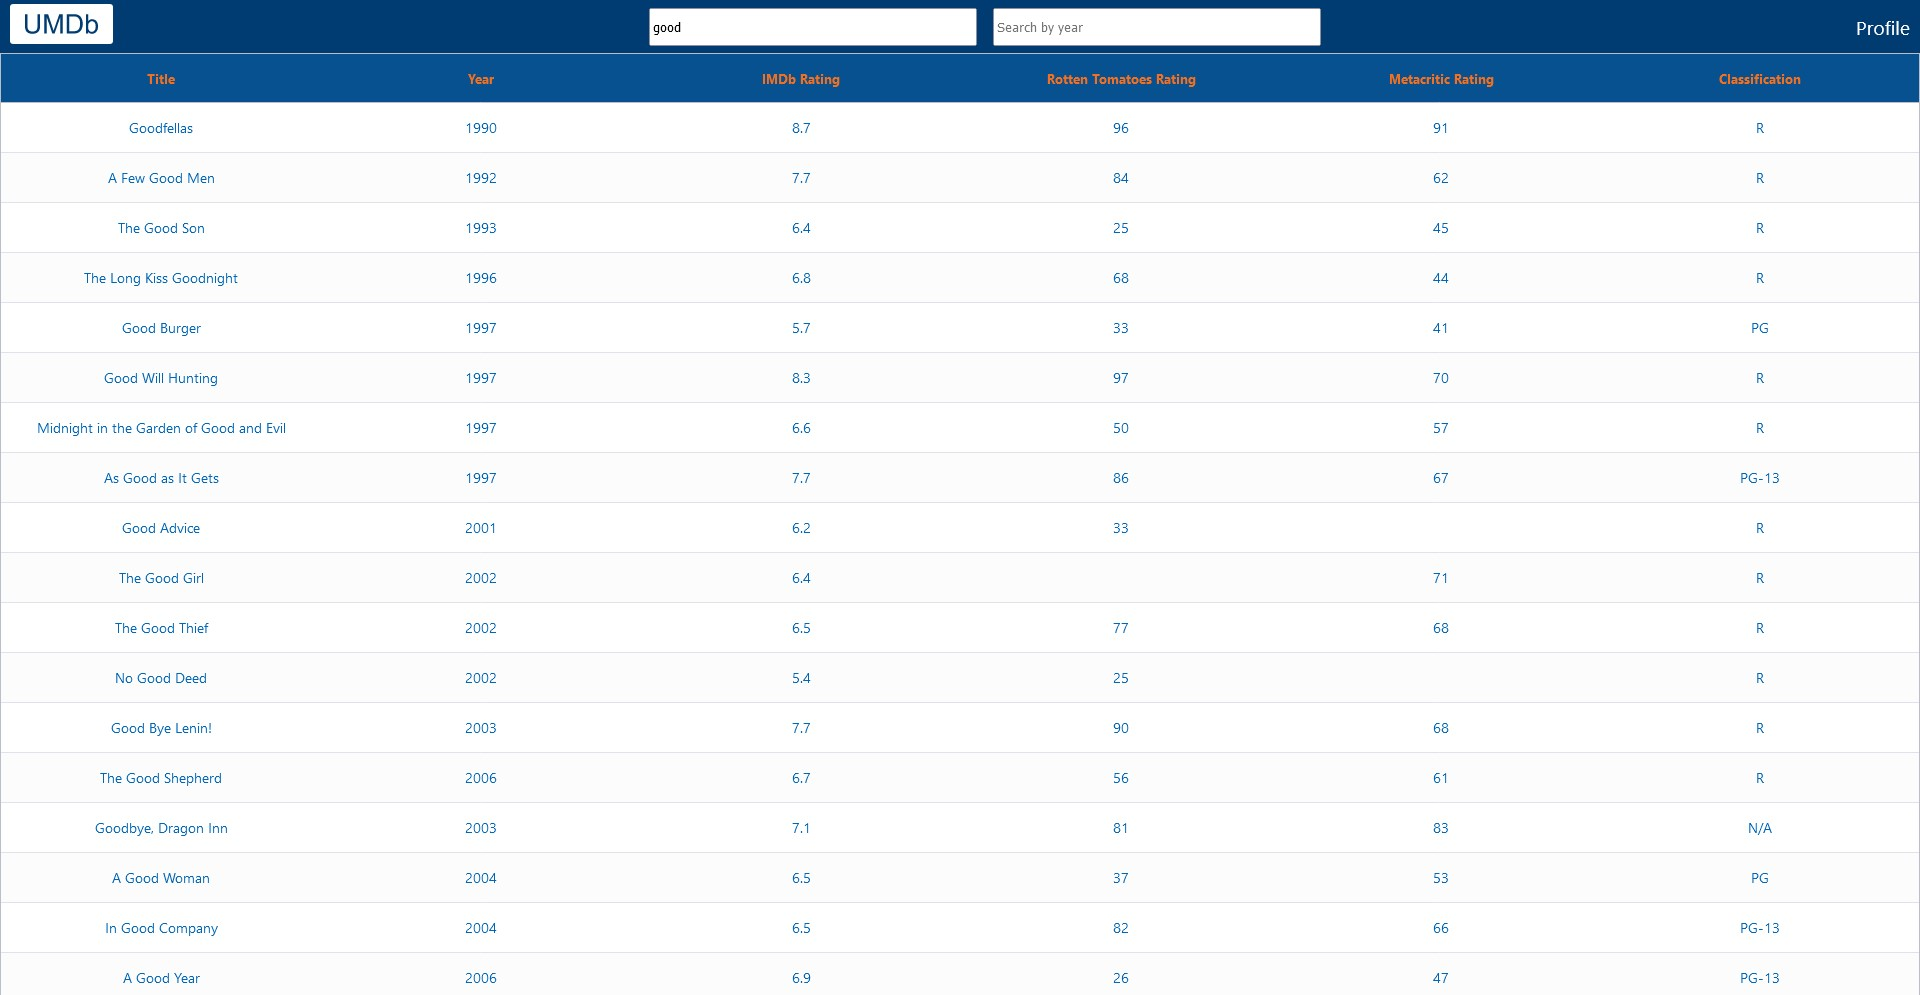
\includegraphics[width=\textwidth]{Figure4.jpg}}
			\end{center}

		\newpage

		\subsection{/people/\{id\}}
			


\end{document}